\chapter{Applications}
\label{chap:applications}


To illustrate the use of the graphical user interface, two different physical
applications are shown in the desktop and the web frontend, respectively. From
the physics point of view, the example in the desktop version focuses more on the
density of states and the visualization of spin contributions, while the dataset
in web frontend focuses on the band structure $E(\mathbf{k})$ and the visualization
of defect states in supercells.

\section{Web Frontend: $\textrm{MoSe}_2$ Crystal}
\label{appl_frontend}

\begin{wrapfigure}{r}{0.4\textwidth} % placed up here cause below would appear
                                % in next section. and in PDF appears next to
                                % matching text.
    \centering
    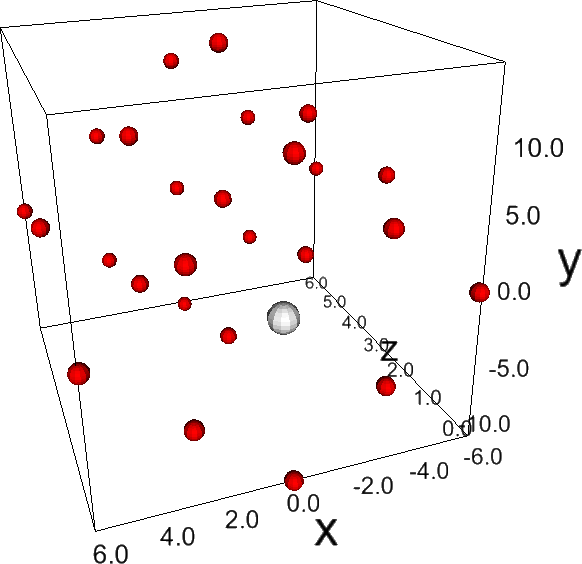
\includegraphics[width=0.38\textwidth]{img/gui_web_mose2_monolayer_atomplot.png}
    \caption[Atom Plot of a $\textrm{MoSe}_2$ monolayer]{Atom plot of a $\textrm{MoSe}_2$ monolayer with the defect atom selected in
      the web frontend}
    \label{fig:modules}
\end{wrapfigure}

Figure \ref{example1} shows the visualization of a band structure calculation of a three-dimensional Molybdenum diselenide ($\textrm{MoSe}_2$ bulk) crystal using the default settings of the GUI. Even with the default settings the band structure plots clearly indicate, that $\textrm{MoSe}_2$ is a semiconductor since there are no states at the Fermi level. Because the minimum of the conduction band is located at another $k$ as the maximum of the valence band, the plot shows that $\textrm{MoSe}_2$ has an indirect band gap. This indicates that for the transition with the smallest energy difference between valence and the conduction band, energy and momentum have to change.

\begin{figure}[htb!]
    \centering
    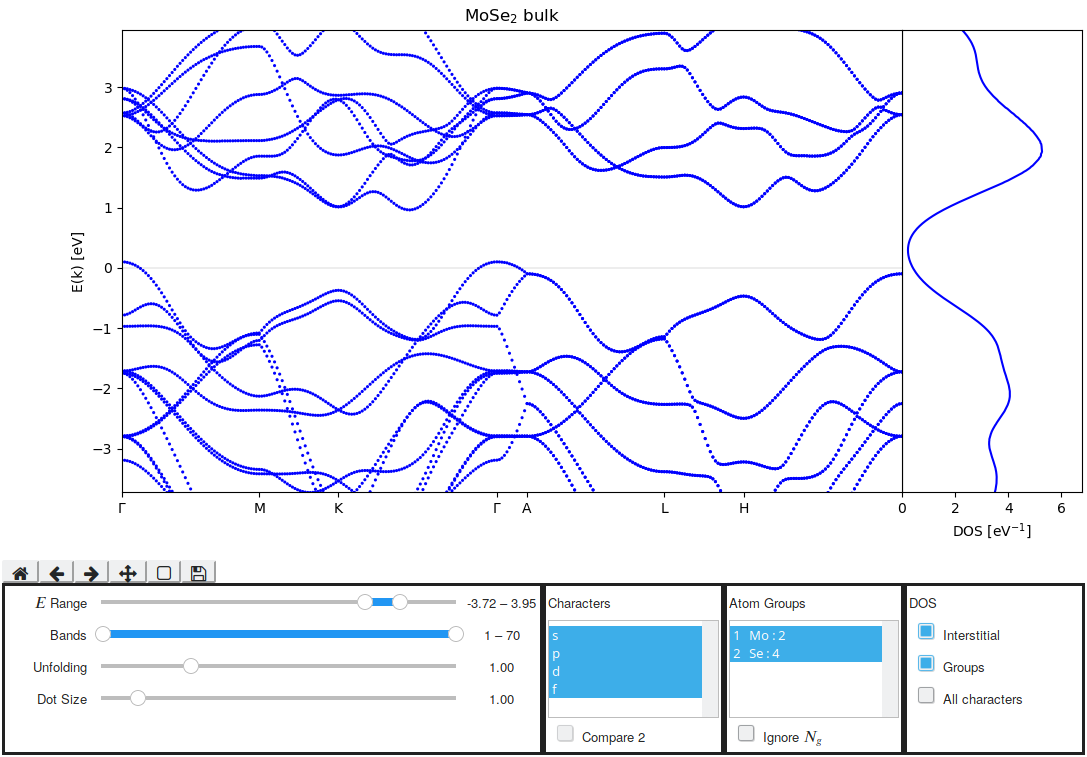
\includegraphics[width=1.0\linewidth]{img/gui_web_mose2_crystal.png}
    \caption[Band structure of a $\textrm{MoSe}_2$ crystal]{Band structure of a $\textrm{MoSe}_2$ crystal using the default settings of the web frontend}
    \label{example1}
\end{figure}

In contrast to the three-dimensional extended $\textrm{MoSe}_2$ crystal, a $\textrm{MoSe}_2$ monolayer (see Fig. \ref{example2}) has a direct band gap but is still a semiconductor. Furthermore, the $\textrm{MoSe}_2$ monolayer has a defect atom in every 9th unit cell and the DFT computation is therefore done in a $3 \times 3$ supercell to restore periodicity. This is the reason for the much greater number of states in the band structure plot. 

\begin{figure}[htb!]
    \centering
    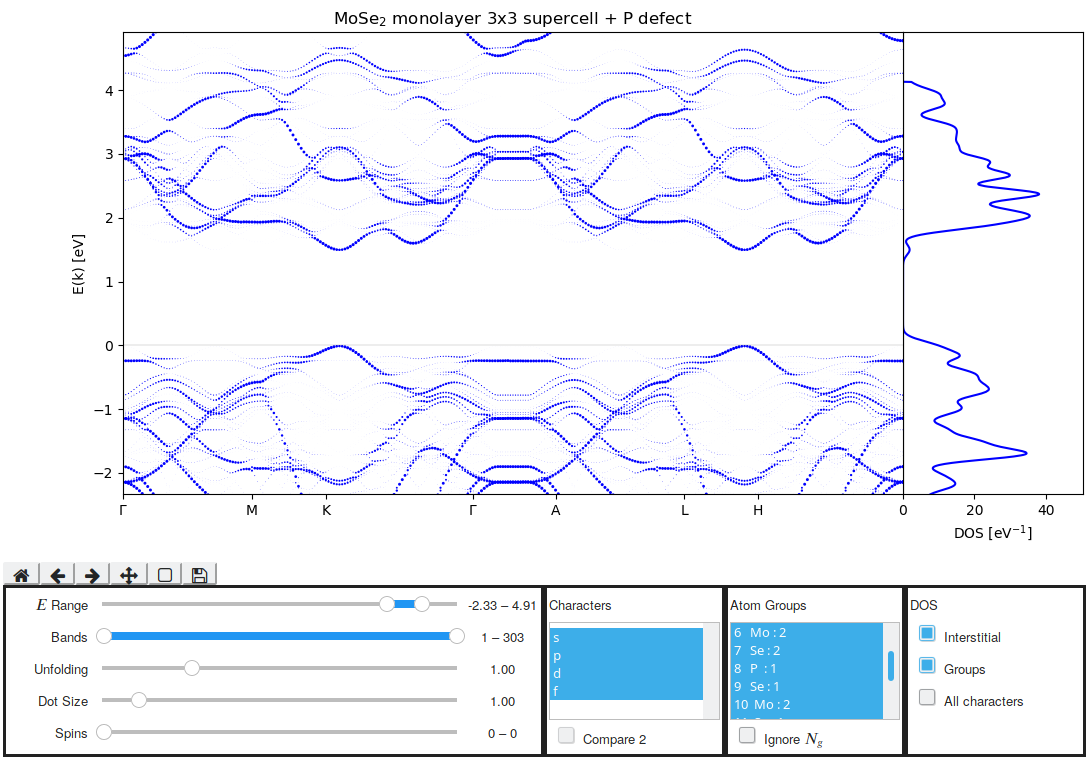
\includegraphics[width=1.0\linewidth]{img/gui_web_mose2_monolayer_unfold-1.png}
    \caption[Band structure of a $\textrm{MoSe}_2$ monolayer]{Band structure of a $\textrm{MoSe}_2$ monolayer using the default settings of the web frontend}
    \label{example2}
\end{figure}

Since the Brillouin zone of the supercell is smaller than the Brillouin zone of the same crystal without the defect, the supercell Brillouin zone is unfolded to the same size as the Brillouin zone of the unperturbed lattice. To account for the fact that the defect is only present in every 9th cell and its relative importance for the spectrum is therefore degraded, an unfolding weight is introduced to visualize the relative importance of bands in the unfolded Brillouin zone. By default, the unfolding weight is used by our visualization tool, but it can gradually be turned off in order to highlight the impact of defect states. This is shown in figure \ref{example3}. To even better visualize the defect state, it would also be possible to select the atom group belonging the defect atom only. In this example, the analysis with reduced band unfolding shows, that there are many more direct band gaps originating from the defect state.


\begin{figure}[htb!]
    \centering
    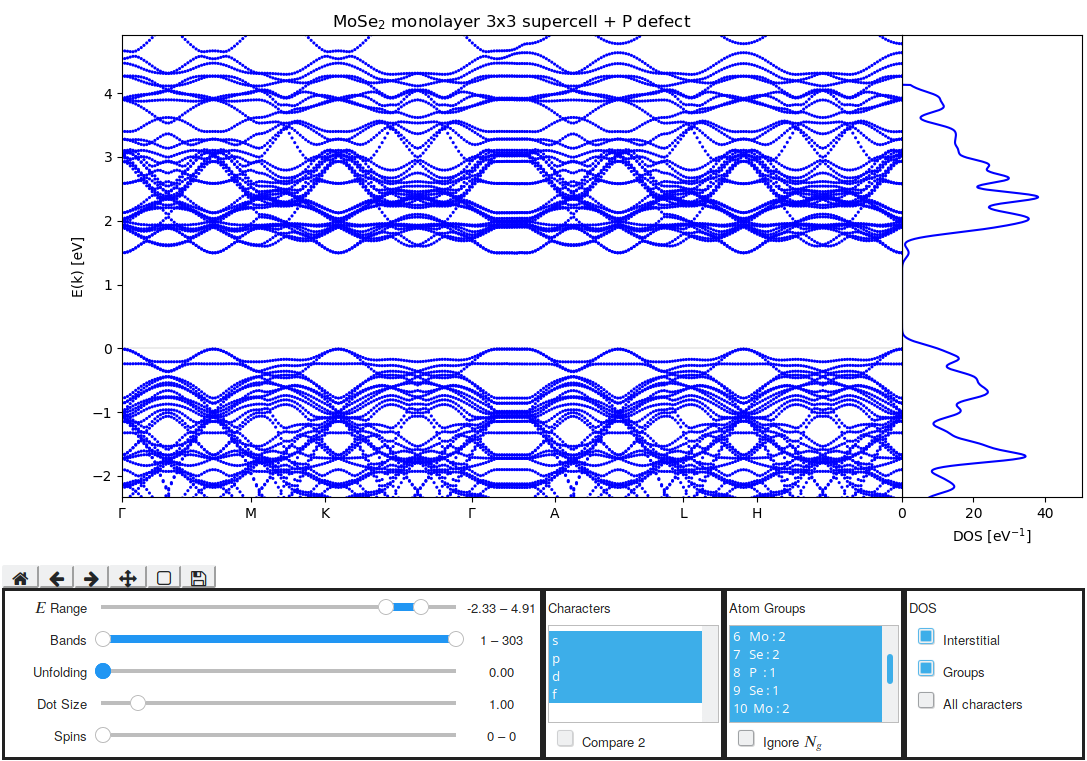
\includegraphics[width=1.0\linewidth]{img/gui_web_mose2_monolayer_unfold-0.png}
    \caption{Band structure of a $\textrm{MoSe}_2$ monolayer without unfolding weights}
    \label{example3}
\end{figure}


\section{Desktop Frontend: $\textrm{Co}$ Crystal}

%% CP: proofread modification v1 of PK Original ========================================
Figure \ref{example4} shows the visualization of a band structure calculation of
a three-dimensional $\textrm{Co}$ crystal with the Desktop frontend. As described in the previous chapters, the possible selections in the Desktop frontend are the same as in the Web frontend and the same \texttt{matplotlib} functions are used to generate the plot, therefore the result looks very similar to the plots in chapter \ref{appl_frontend}. Since Cobalt is a ferromagnet, it is interesting to investigate the spin dependence of the bands and the density of states. Therefore, for \ref{example4} the default settings of the GUI were modified to show both spins. As there are no defect atoms involved in this example, there is no need to perform a supercell calculation. Therefore, we do not have an unfolding weight here. 

A quick look at \ref{example4} shows that there are several bands that intersect with the Fermi level. This indicates that in contrast to the $\textrm{MoSe}_2$ example, electrons can be easily excited in the conduction band without a band gap, which makes $\textrm{Co}$ is a conductor.

The density of states plotted next to the band structure plot encrypts the available number of states for each spin at energy E. Since the system always minimizes its energy, only states up to the Fermi level are occupied. Counting the number of occupied states for both spins shows an excess of blue spins over the red spins. This indicates, that the $\textrm{Co}$ crystal has a net magnetic dipole moment, that contributes to the magnetic properties of Cobalt. This supports the well-known fact that Cobalt is a ferromagnetic material.

These are two properties which were deduced by observing the band-DOS plot, but
depending on the material and band-DOS plot many properties can be extracted and
derived.

\begin{figure}[htb!]
    \centering
    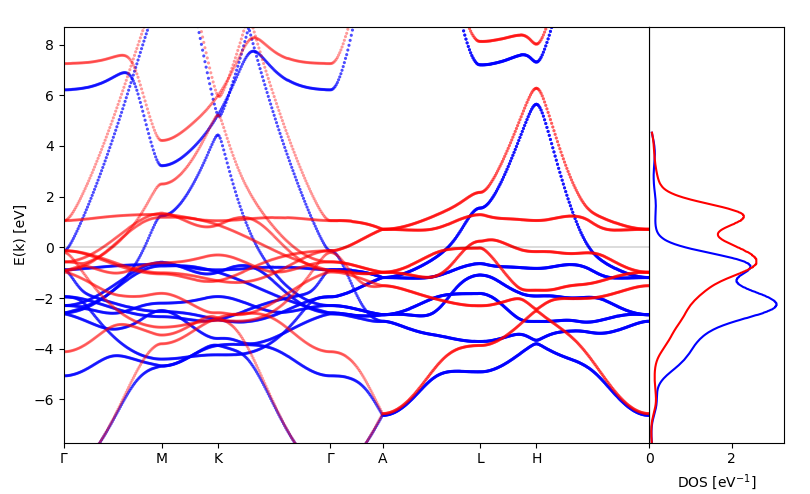
\includegraphics[width=0.7\linewidth]{fig/image1.png}
    \caption[Band structure of a $\textrm{Co}$ crystal]{Band structure of a $\textrm{Co}$
      crystal in the desktop frontend. The density of states indicates a net magnetic moment in the crysal}
    \label{example4}
\end{figure}



% %% PK Original ========================================
% Figure \ref{example4} shows the visualization of a band structure calculation of
% a three-dimensional $\textrm{Co}$ crystal with the selection both spins, one
% atom group (since it is the only crystal in the cell structure) with all characters and whole band selected with exponent being at $0.0$. We can see in the figure that band plot of any spin intersecting with the Fermi energy level. This means that many electrons excite to valance band which is a characteristic of a conductor. Hence the Co Crystal can be considered and concluded as conductor material.

% One more physical property of Co crystal can be determined by considering and reading the density of state(DOS) files and plotting the density of state along with the band plots. In the figure \ref{example4}, on the right one can see the Density of states of both the spins. If the area covered under the density is considered, it is clear that under the Fermi energy, electrons of one spin covers more area than other spin in the density of states plot. This means there are more electrons with positive spin under the Fermi energy. This is the character exhibited by the Ferro magnetic substance, so it be considered and concluded that this Co crystal is a Ferro magnetic.

% There are two properties which are concluded by observing the band-dos plot but depending on the material and band-dos plot many properties can be extracted and concluded.
% \begin{figure}[htb!]
%     \centering
%     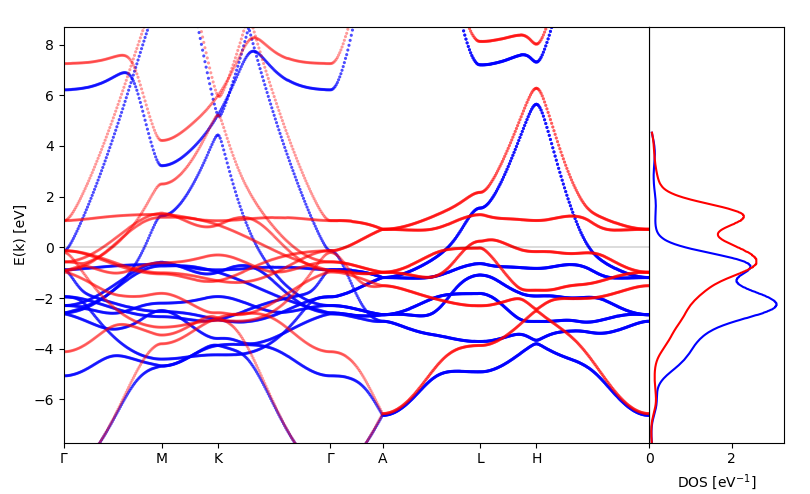
\includegraphics[width=0.7\linewidth]{fig/image1.png}
%     \caption[Band structure of a $\textrm{Co}$ ]{Band structure of a $\textrm{Co}$ using the above settings of the Desktop frontend}
%     \label{example4}
% \end{figure}



\section{Derived physical Quantities: Differentiation}
\label{sec:deriv-phys-quant}
% bänder isonlieren schwierig....fleur update--> label der E eigenvlas

%$m^{*}$ and $v_{G}(\mathbf{k})$


The kind of datasets handled in the scope of the project did not lend themselves
readily to applications of automatic differentiation techniques. Nevertheless,
it is possible to derive meaningful physical quantities from the band structure
using numerical differentiation techniques.

The effective mass $m^{*}$ represents the mass, that an electron appears to have due to the inter-atomic forces in the crystal. At every $\mathbf{k}_0$, where $E(\mathbf{k})$ has a local extremum, $E(\mathbf{k})$ can be expanded in a Taylor series with a vanishing first order term $E(\mathbf{k}) = E_0 + \frac{\partial E(\mathbf{k})}{\partial \mathbf{k}} \cdot (\mathbf{k}-\mathbf{k}_0)^2$. Comparing this to the dispersion relation of a free electron $E(\mathbf{k})_{free} = \frac{\hbar^2 \mathbf{k}^2}{2 m_e}$ motivates the general definition 

\begin{equation}
    m^{*}_{k_i,k_j} = \hbar^2  \left(\frac{\partial^2E(\mathbf{k})}{\partial k_i \partial k_j}\right)^{-1}
\end{equation}

Since $\frac{\partial^2E(\mathbf{k})}{\partial \mathbf{k}_i \partial \mathbf{k}_j}$ depends on the direction of the partial derivatives, $m^{*}_{k_i,k_j}$ is a tensor. Because the band structure files only contain a discretely sampled path in the Brillouin zone, only the derivatives that correspond to the direction from one high-symmetry point to the next can be computed. We are only interested in the diagonal terms of $m^{*}\big|_{i,j}$.

%maybe something about the directional dependency --> m is tensor...


A second potentially interesting quantity is the group velocity $v_{G}(\mathbf{k})$ associated to each band. The group velocity $v_{G}(\mathbf{k})$ at the Fermi energy $E = E_F$ is called Fermi velocity.

\begin{equation}
    v_{G}(\mathbf{k})_{k_i} = \frac{1}{\hbar}\frac{\partial E(\mathbf{k})}{\partial \mathbf{k_i}}
\end{equation}


\subsection{Differentiation}

Since the k-mesh in DFT calculations is potentially very sparse, low order finite difference schemes are not expected to work well. Alternatively, one way to exploit all data points efficiently is to use fast Fourier transform methods, which are equivalent to the derivation of a truncated Fourier series. This method is expected to be well-suited for the problem since the graph of the band structure $(k, E(|k|))$ with $k \in \left[-\Gamma, H, \Gamma \right) $ is periodic, where $\Gamma$ and $H$ are arbitrary representatives of the high symmetry points. This periodicity in the reciprocal space is a direct consequence of the periodicity of the crystal.

In Fourier space, spatial derivatives transform into multiplications, which can easily be shown by partial integration.

\begin{equation}
    f^{(n)}(x) = \mathcal{F}^{-1}\left((ik)^n\mathcal{F}(f(x))\right)
\end{equation}
 
To test the FFT differentiation method, a band was selected that did not have intersections with other bands within the interval between two high symmetry points. Then a resolution study was done to investigate the impact of the number of points within the interval.
% and a stationary point at the high symmetry points
The comparison between the FFT and a first-order central difference approximation of the second derivative (FD) is shown in Fig. \ref{num_diff}, where different k-mesh resolutions are compared to a derivative that is almost fully converged. The comparison indicates that for small N, the error of the FFT method is significantly smaller than the error of the FD derivative. This is especially striking in the vicinity of the high symmetry points, where the error of the differentiation is required to be small in order to get good approximations for $m^{*}$, which is only meaningful close to the high symmetry points.


\begin{figure}[htb!]
    \centering
    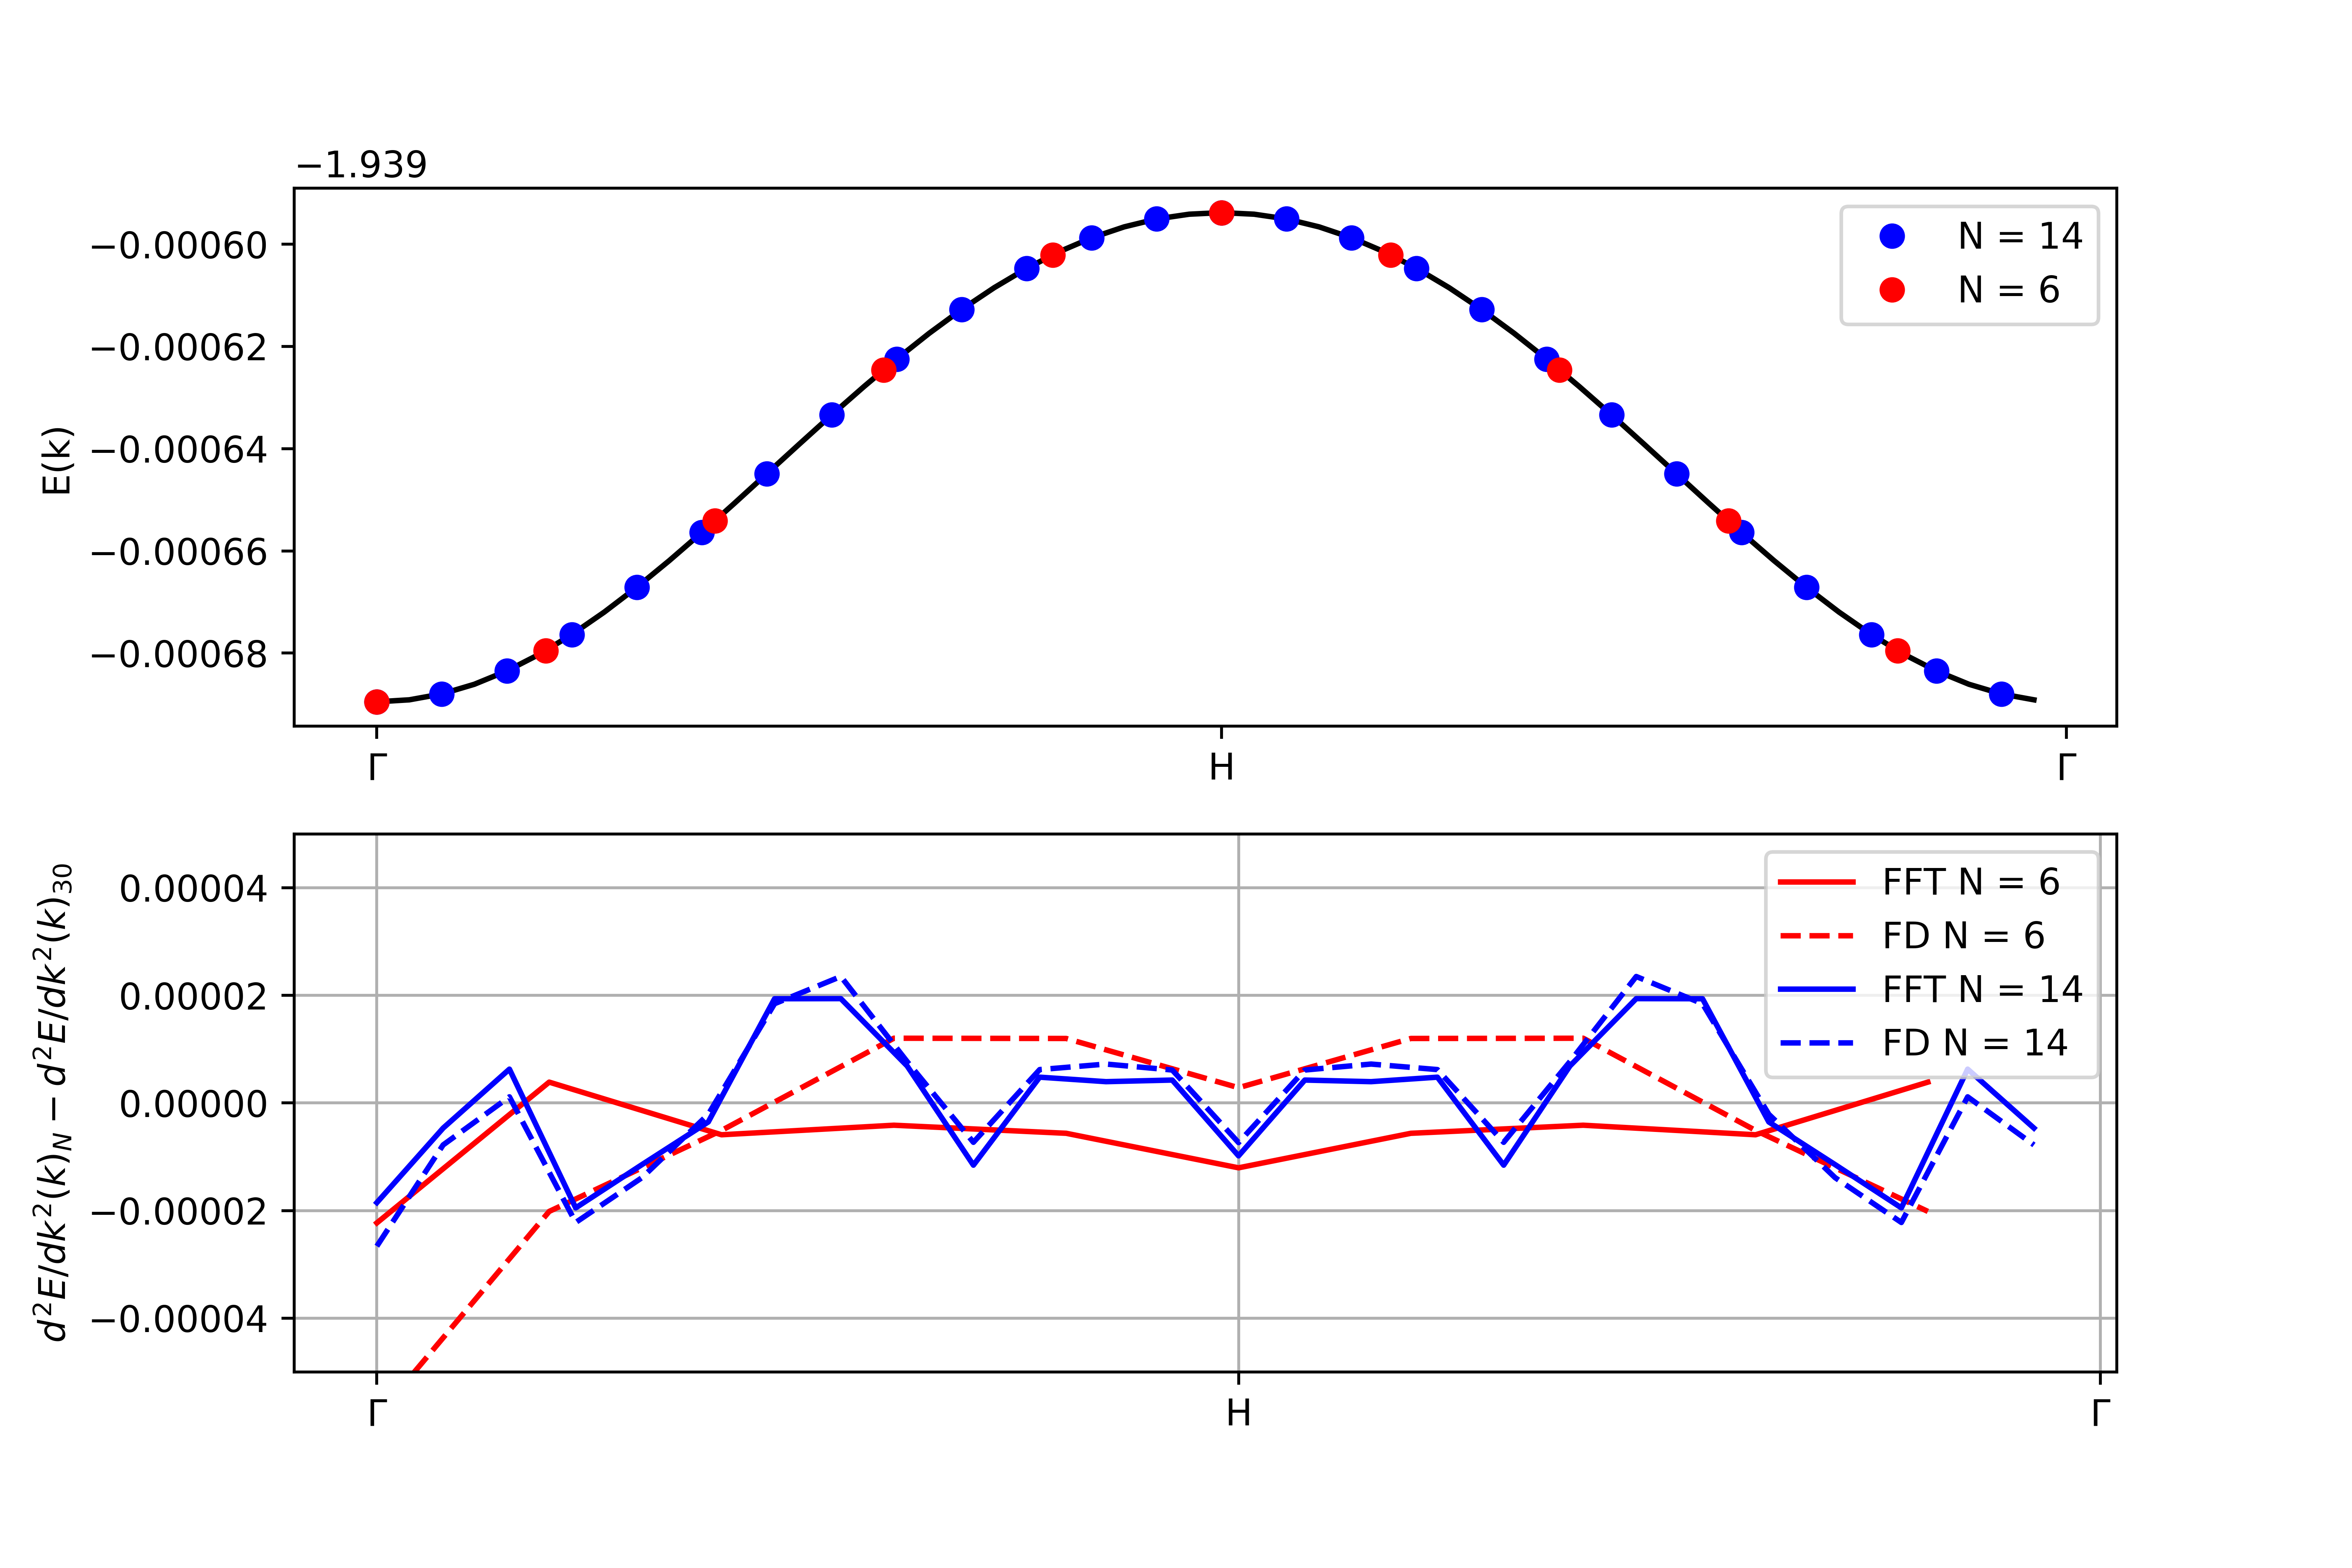
\includegraphics[width=0.7\linewidth]{christian/diff_compare.png}
    \caption{Comparison between FFT differentiation method and central finite difference method}
    \label{num_diff}
\end{figure}

When using more points, the difference between both approximation schemes is not significant. It is interesting to note, that the FFT method does not work anymore in the limit of extremely many points. In this case, the derivative is dominated by Gibbs oscillations. These are most likely caused by small discontinuities in $E(\mathbf{k})$, due to the different basis size at each k point in the DFT computation.

At the current state, the question remains to be answered whether the computation of $m^{*}$ and $v_g$ is useful. The number of bands, which the computation can be applied to is extremely limited. Since the bands in the data files are not labeled according to their corresponding eigenfunction but sorted by value, there are discontinuities at each point, where two bands intersect. This problem might be solved in the future. 













 %   \item Effective mass, that an electon in a crystal appears to have compared to a free %electron (due to interactions in the solid)
%    $m^{*} = \hbar^2  \left(\frac{\partial^2E(\mathbf{k})}{\partial k^2}\right)^{-1}$
%    \
%    \item Group velocity:
%    $v_{G}(\mathbf{k}) = \frac{1}{\hbar}\frac{\partial E(\mathbf{k})}{\partial \mathbf{k}}$%
%
%    
%    \item Problem: sparse k-Point mesh, but periodic band structure
%    \item Idea: Using FFT to compute accurate derivates:
%    \newline $\Leftrightarrow$ Differentiate a finite Fourier series
%    \newline $f^{(n)}(x) = \mathcal{F}^{-1}\left((ik)^n\mathcal{F}(f(x))\right)$


%%% Local Variables:
%%% mode: latex
%%% TeX-master: "../report"
%%% End:

%  LocalWords:  supercells
